\chapter{Some LaTeX examples}
This chapter includes examples of how to do common tasks using LaTeX{}. Although most users will be familiar with these commands and environments, these serve as a) a test of the class file and conversion process, and b) examples that are known to work with the class and conversion process. So, when all else fails, users can copy these examples and tailor them to their particular case.

\section{Headings}
LaTeX{} allows a very simple definition of the document's structure. This document has the following structure:
\begin{itemize}
\item Chapter 1: what is LaTeX?
\begin{itemize}
\item Section 1: Headings
\item Section 2: Floats
\item Section 3: Mathematics
\item Section 4: Lists
\end{itemize}
\item etc. \ldots
\end{itemize}

\subsection{Chapter}
To define a new chapter, simply write \verb+\chapter{What is LaTeX?}+.

To use chapters, pass the \texttt{memoir}, \texttt{book}, or \texttt{report} option to \emph{nrel.cls} (see Section \ref{sec:nrel.cls.options}).

\subsection{Sections}
If Chapters are the highest level headings in a document, sections come next, followed by subsections. Although there don't have to be chapters in a document, a LaTeX document does need to have Sections.

So: 

\begin{verbatim}
\section{Headings}
LaTeX{} allows a very simple definition of the document's structure. 
This document has the following structure:
...
\subsection{Chapter}

\end{verbatim}

\section{Body text}
Body text does not need to be specially identified in LaTeX{}. Non-printing comments are identified in the source document(s) using the \% symbol.

\section{Mathematics}

LaTeX is great at typesetting mathematics. The following example is taken from the \href{www.writelatex.com}{www.writelatex.com} website:

\begin{quote}
Making inline equations is easy. Let $X_1, X_2, \ldots, X_n$ be a sequence of independent and identically distributed random variables with $\textrm{E}[X_i] = \mu$ and $\textrm{Var}[X_i] = \sigma^2 < \infty$, and let
$$S_n = \frac{X_1 + X_2 + \cdots + X_n}{n}
 = \frac{1}{n}\sum_{i}^{n} X_i$$
denote their mean. Then as $n$ approaches infinity, the random variables $\sqrt{n}(S_n - \mu)$ converge in distribution to a normal $\mathcal{N}(0, \sigma^2)$.
\end{quote}

Alternatively, if numbered equations are required, use the \texttt{equation} environment. For example:

\begin{verbatim}
\begin{equation}
y = mx +c \textrm{.}
\label{eqn:line}
\end{equation}
\end{verbatim}

would give:

\begin{equation}
y = mx+c \textrm{.}
\label{eqn:line}
\end{equation}

\section{Cross references}
Use labels and references to refer back and forth to figures, equations, tables and sections. For example, \verb+Eqn. \ref{eqn:line}+ gives a reference to Eqn. \ref{eqn:line}.

\section{Floats}
Floats are images, tables or other pieces of the document that are free to move to the best place in the document for them. Literally, they `float'. The two most common floats are the tabular environment (for tables) and the figure environment for figures.

\subsection{Tables}
Use the \texttt{tabular} environment to produce basic tables. Table~\ref{tab:widgets} is produced using this code: 

\begin{verbatim}
\begin{table}[!h]
\centering
\caption{An example table.}\label{tab:widgets}
\begin{tabular}{lr}
Item & Quantity \\\hline
Widgets & 42 \\
Gadgets & 13
\end{tabular}
\end{table}
\end{verbatim}

\begin{table}[!h]
\centering
\caption{An example table.}\label{tab:widgets}
\begin{tabular}{lr}
Item & Quantity \\\hline
Widgets & 42 \\
Gadgets & 13
\end{tabular}
\end{table}

Resist the temptation to stop table rows early. If all of the delimiters  (\&) are included in each row, the table will be complete and will better translate to RTF later.

\subsection{Figures}
To include a figure in a document, use the \texttt{figure} environment and the \texttt{includegraphics} command.

\begin{verbatim}
\begin{figure}
\includegraphics[width=\textwidth]{figure's-file-name}
\caption{Caption goes here.}\label{fig:figuresLabel}
\end{figure}
\end{verbatim}

\subsection{Subfigures}
Subfigures are implemented using the \texttt{subfig} package. Although this package is deprecated (apparently \texttt{subcaption} is now the preferred package), it plays fairly nicely with \texttt{latex2rtf} so will be used for the foreseeable future. 

The \texttt{label}s in the example below allow us to make references using the \texttt{ref} command, both to the overall figure (Figure \ref{fig:NRELimages}) and the subfigures (Figures \ref{fig:21206} and \ref{fig:20018}) directly. Unfortunately, \texttt{latex2rtf} does not allow multiple \texttt{label}s in a Figure environment, and so only the first label will be kept: therefore, it's best to just use a single label in any one \texttt{figure} environment.

\begin{verbatim}
\begin{figure}
\centering
\hfill
\subfigure[Wind turbines at the Forward Wind Energy Center in Fond du Lac 
 and Dodge Counties, Wisconsin. (Photo by Ruth Baranowski / NREL)
 \label{fig:21206}]{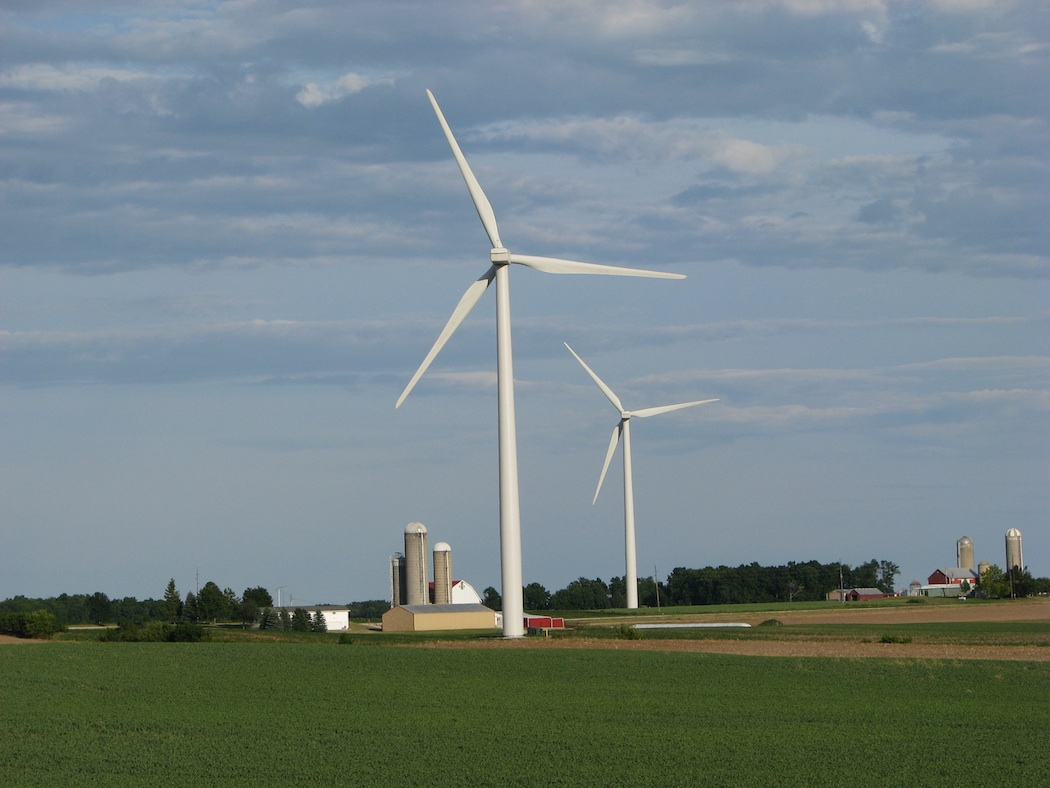
\includegraphics[height=2.5in]{files/21206}}
\hfill 
\subfigure[Aerial view of the National Wind Technology Center. 
 (Photo by Dennis Schroeder / NREL)\label{fig:20018}]
 {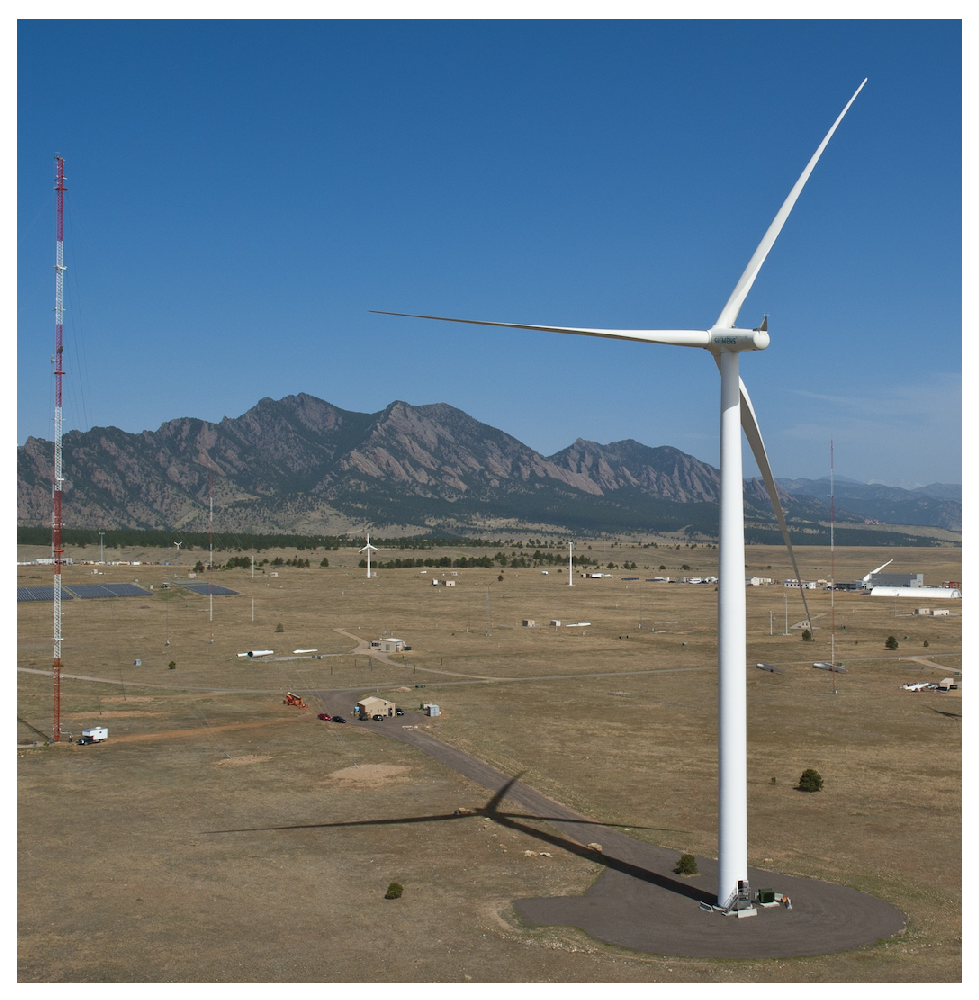
\includegraphics[height=2.5in]{files/20018}}
\hfill
\caption{NREL images}\label{fig:NRELimages}
\end{figure}
\end{verbatim}
 
\begin{figure*}[htp]
\centering
\hfill
\subfigure[Wind turbines at the Forward Wind Energy Center in Fond du Lac and Dodge Counties, Wisconsin. (Photo by Ruth Baranowski / NREL)\label{fig:21206}]{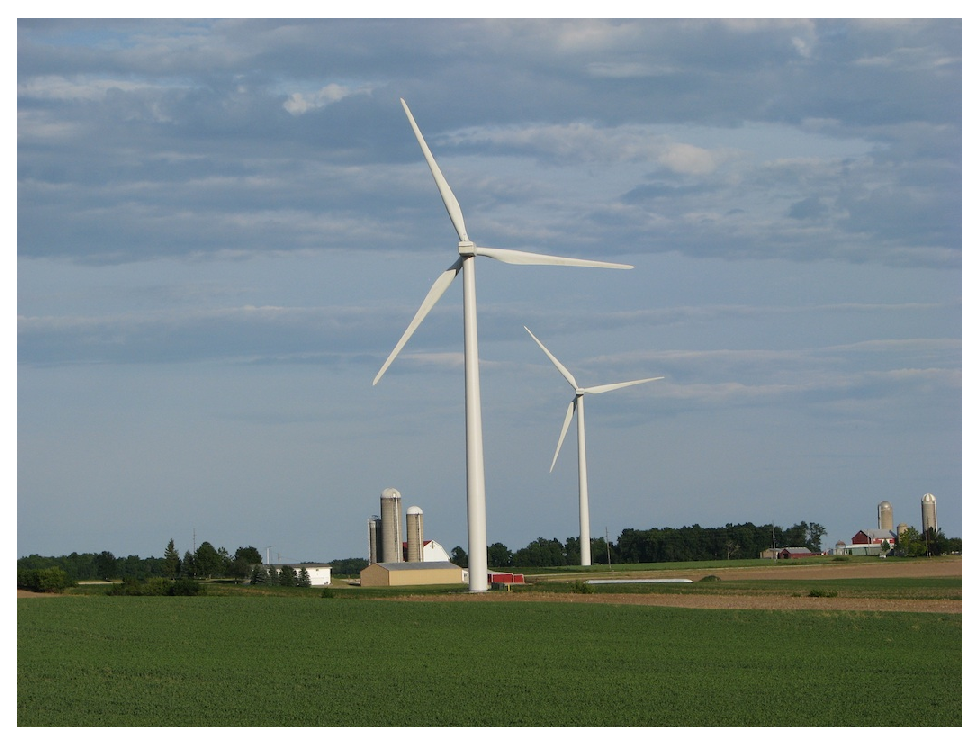
\includegraphics[height=2.5in]{files/21206.eps}}
~ %add desired spacing between images, e. g. ~, \quad, \qquad etc. (or a blank line to force the subfigure onto a new line)
\hfill
\subfigure[Aerial view of the National Wind Technology Center. (Photo by Dennis Schroeder / NREL)\label{fig:20018}]{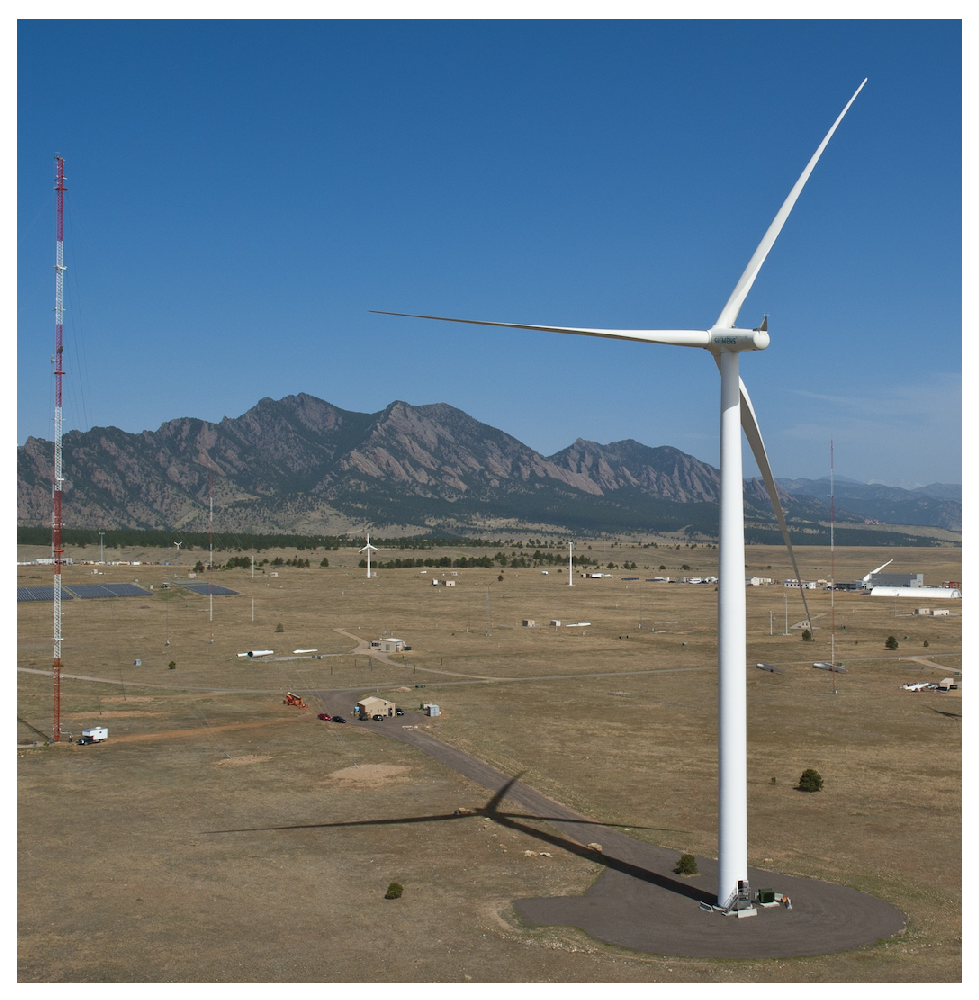
\includegraphics[height=2.5in]{files/20018.eps}}
\hfill
\caption{NREL images}\label{fig:NRELimages}
\end{figure*}

If a subfigure is split over two lines using \verb+\\+, make sure those symbols are on their own line.

\section{Lists}

To make lists with automatic numbering, use the \texttt{enumerate} environment:

\begin{enumerate}
\item Like this,
\item and like this.
\end{enumerate}
\dots or bullet points \dots
\begin{itemize}
\item Like this,
\item and like this.
\end{itemize}

\section{Computer code}
The \texttt{lstlisting} package has been loaded.

\section{Creating a file structure}
\label{sec:FileStructure}
Use the \texttt{input} command to import other files into your main file. For example, each of the chapters in this report could be in separate files, called \emph{NRELRequirements} (Chapter 1), \emph{LatexAtNREL} (Chapter 2), and so-on. 

\begin{verbatim}
...
% content
\input{NRELRequirements}
\input{LatexAtNREL}
\chapter{Some LaTeX examples}
This chapter includes examples of how to do common tasks using LaTeX{}. Although most users will be familiar with these commands and environments, these serve as a) a test of the class file and conversion process, and b) examples that are known to work with the class and conversion process. So, when all else fails, users can copy these examples and tailor them to their particular case.

\section{Headings}
LaTeX{} allows a very simple definition of the document's structure. This document has the following structure:
\begin{itemize}
\item Chapter 1: what is LaTeX?
\begin{itemize}
\item Section 1: Headings
\item Section 2: Floats
\item Section 3: Mathematics
\item Section 4: Lists
\end{itemize}
\item etc. \ldots
\end{itemize}

\subsection{Chapter}
To define a new chapter, simply write \verb+\chapter{What is LaTeX?}+.

To use chapters, pass the \texttt{memoir}, \texttt{book}, or \texttt{report} option to \emph{nrel.cls} (see Section \ref{sec:nrel.cls.options}).

\subsection{Sections}
If Chapters are the highest level headings in a document, sections come next, followed by subsections. Although there don't have to be chapters in a document, a LaTeX document does need to have Sections.

So: 

\begin{verbatim}
\section{Headings}
LaTeX{} allows a very simple definition of the document's structure. 
This document has the following structure:
...
\subsection{Chapter}

\end{verbatim}

\section{Body text}
Body text does not need to be specially identified in LaTeX{}. Non-printing comments are identified in the source document(s) using the \% symbol.

\section{Mathematics}

LaTeX is great at typesetting mathematics. The following example is taken from the \href{www.writelatex.com}{www.writelatex.com} website:

\begin{quote}
Making inline equations is easy. Let $X_1, X_2, \ldots, X_n$ be a sequence of independent and identically distributed random variables with $\textrm{E}[X_i] = \mu$ and $\textrm{Var}[X_i] = \sigma^2 < \infty$, and let
$$S_n = \frac{X_1 + X_2 + \cdots + X_n}{n}
 = \frac{1}{n}\sum_{i}^{n} X_i$$
denote their mean. Then as $n$ approaches infinity, the random variables $\sqrt{n}(S_n - \mu)$ converge in distribution to a normal $\mathcal{N}(0, \sigma^2)$.
\end{quote}

Alternatively, if numbered equations are required, use the \texttt{equation} environment. For example:

\begin{verbatim}
\begin{equation}
y = mx +c \textrm{.}
\label{eqn:line}
\end{equation}
\end{verbatim}

would give:

\begin{equation}
y = mx+c \textrm{.}
\label{eqn:line}
\end{equation}

\section{Cross references}
Use labels and references to refer back and forth to figures, equations, tables and sections. For example, \verb+Eqn. \ref{eqn:line}+ gives a reference to Eqn. \ref{eqn:line}.

\section{Floats}
Floats are images, tables or other pieces of the document that are free to move to the best place in the document for them. Literally, they `float'. The two most common floats are the tabular environment (for tables) and the figure environment for figures.

\subsection{Tables}
Use the \texttt{tabular} environment to produce basic tables. Table~\ref{tab:widgets} is produced using this code: 

\begin{verbatim}
\begin{table}[!h]
\centering
\caption{An example table.}\label{tab:widgets}
\begin{tabular}{lr}
Item & Quantity \\\hline
Widgets & 42 \\
Gadgets & 13
\end{tabular}
\end{table}
\end{verbatim}

\begin{table}[!h]
\centering
\caption{An example table.}\label{tab:widgets}
\begin{tabular}{lr}
Item & Quantity \\\hline
Widgets & 42 \\
Gadgets & 13
\end{tabular}
\end{table}

Resist the temptation to stop table rows early. If all of the delimiters  (\&) are included in each row, the table will be complete and will better translate to RTF later.

\subsection{Figures}
To include a figure in a document, use the \texttt{figure} environment and the \texttt{includegraphics} command.

\begin{verbatim}
\begin{figure}
\includegraphics[width=\textwidth]{figure's-file-name}
\caption{Caption goes here.}\label{fig:figuresLabel}
\end{figure}
\end{verbatim}

\subsection{Subfigures}
Subfigures are implemented using the \texttt{subfig} package. Although this package is deprecated (apparently \texttt{subcaption} is now the preferred package), it plays fairly nicely with \texttt{latex2rtf} so will be used for the foreseeable future. 

The \texttt{label}s in the example below allow us to make references using the \texttt{ref} command, both to the overall figure (Figure \ref{fig:NRELimages}) and the subfigures (Figures \ref{fig:21206} and \ref{fig:20018}) directly. Unfortunately, \texttt{latex2rtf} does not allow multiple \texttt{label}s in a Figure environment, and so only the first label will be kept: therefore, it's best to just use a single label in any one \texttt{figure} environment.

\begin{verbatim}
\begin{figure}
\centering
\hfill
\subfigure[Wind turbines at the Forward Wind Energy Center in Fond du Lac 
 and Dodge Counties, Wisconsin. (Photo by Ruth Baranowski / NREL)
 \label{fig:21206}]{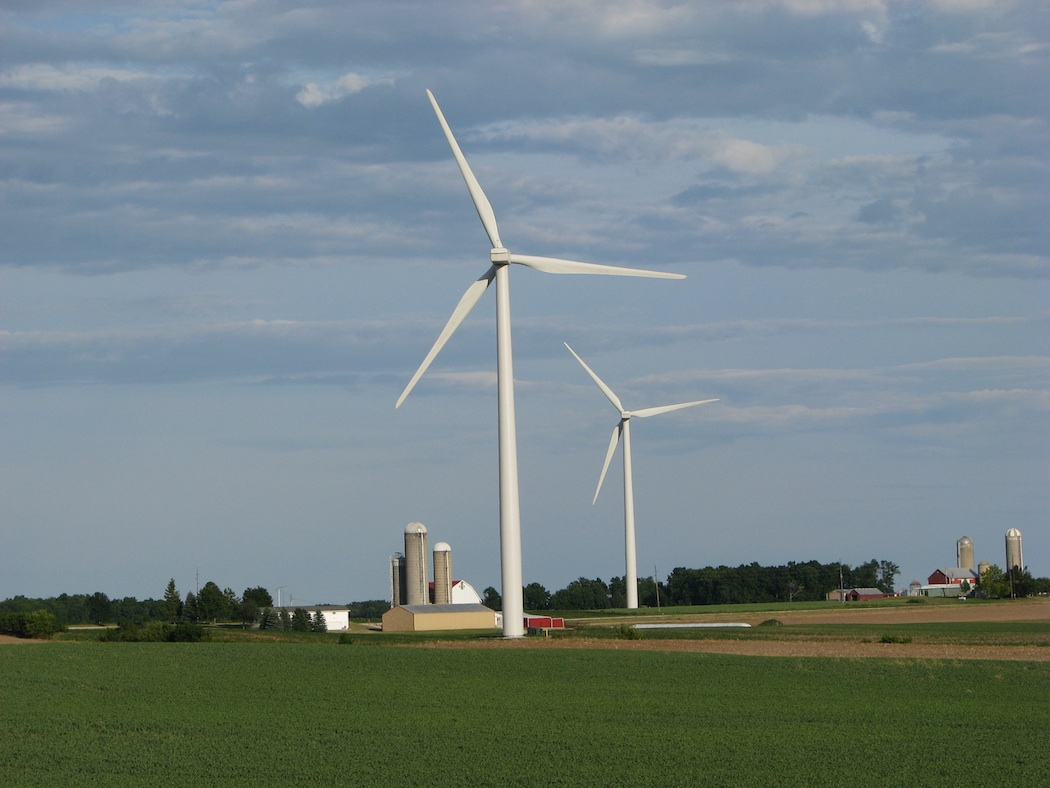
\includegraphics[height=2.5in]{files/21206}}
\hfill 
\subfigure[Aerial view of the National Wind Technology Center. 
 (Photo by Dennis Schroeder / NREL)\label{fig:20018}]
 {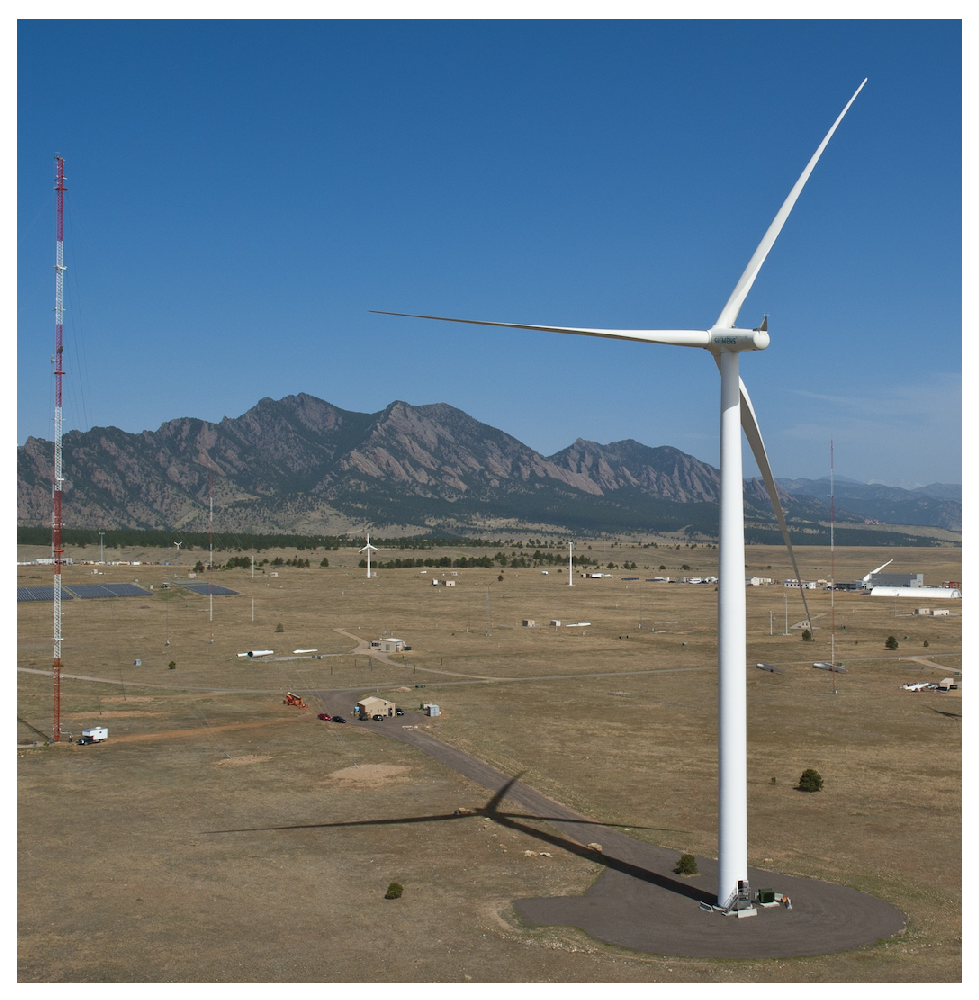
\includegraphics[height=2.5in]{files/20018}}
\hfill
\caption{NREL images}\label{fig:NRELimages}
\end{figure}
\end{verbatim}
 
\begin{figure*}[htp]
\centering
\hfill
\subfigure[Wind turbines at the Forward Wind Energy Center in Fond du Lac and Dodge Counties, Wisconsin. (Photo by Ruth Baranowski / NREL)\label{fig:21206}]{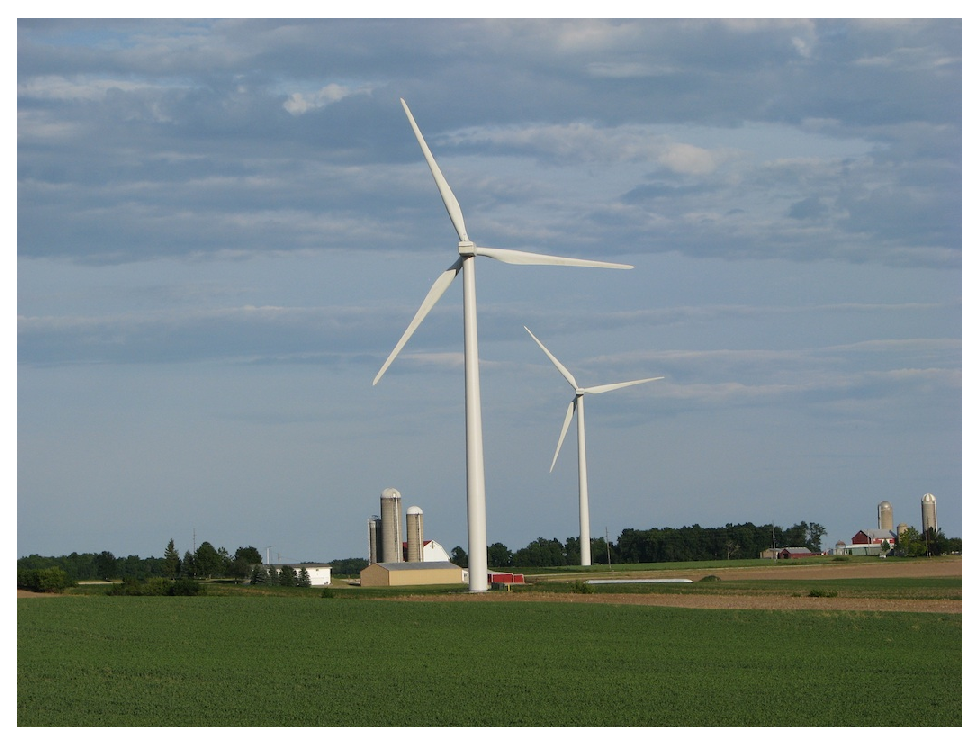
\includegraphics[height=2.5in]{files/21206.eps}}
~ %add desired spacing between images, e. g. ~, \quad, \qquad etc. (or a blank line to force the subfigure onto a new line)
\hfill
\subfigure[Aerial view of the National Wind Technology Center. (Photo by Dennis Schroeder / NREL)\label{fig:20018}]{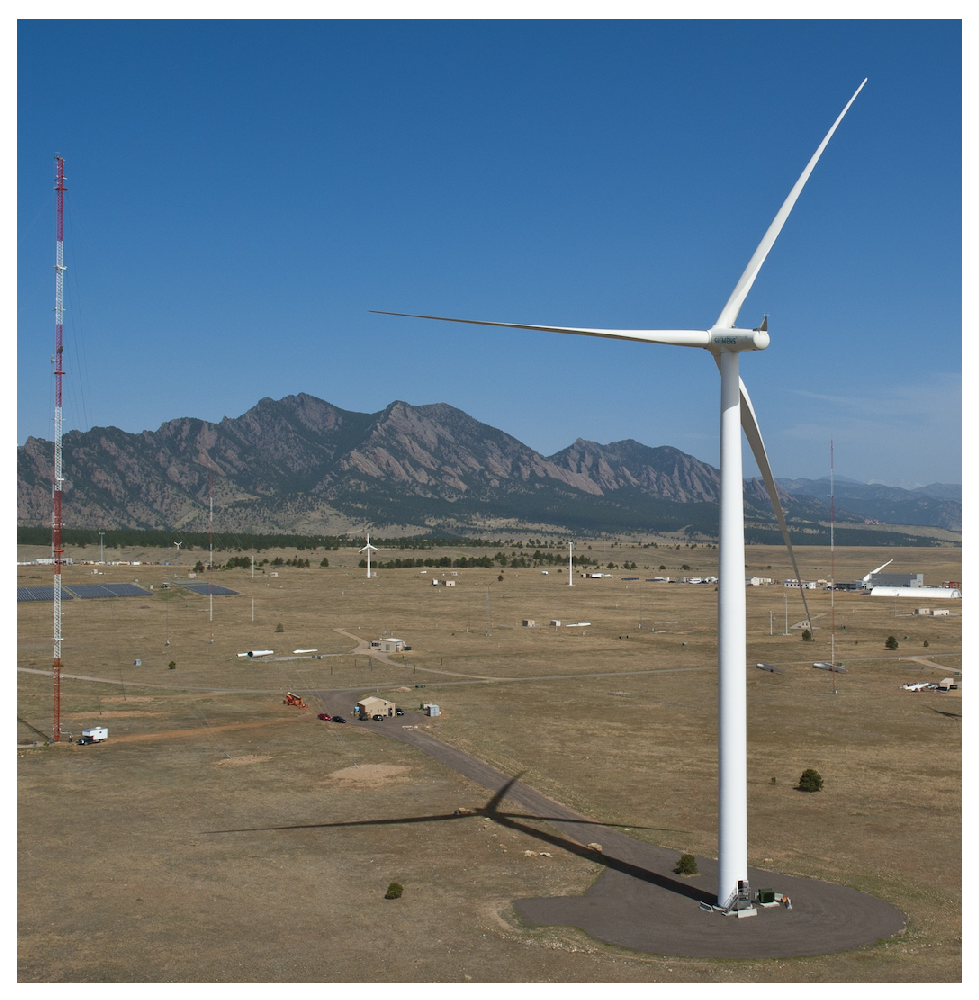
\includegraphics[height=2.5in]{files/20018.eps}}
\hfill
\caption{NREL images}\label{fig:NRELimages}
\end{figure*}

If a subfigure is split over two lines using \verb+\\+, make sure those symbols are on their own line.

\section{Lists}

To make lists with automatic numbering, use the \texttt{enumerate} environment:

\begin{enumerate}
\item Like this,
\item and like this.
\end{enumerate}
\dots or bullet points \dots
\begin{itemize}
\item Like this,
\item and like this.
\end{itemize}

\section{Computer code}
The \texttt{lstlisting} package has been loaded.

\section{Creating a file structure}
\label{sec:FileStructure}
Use the \texttt{input} command to import other files into your main file. For example, each of the chapters in this report could be in separate files, called \emph{NRELRequirements} (Chapter 1), \emph{LatexAtNREL} (Chapter 2), and so-on. 

\begin{verbatim}
...
% content
\input{NRELRequirements}
\input{LatexAtNREL}
\chapter{Some LaTeX examples}
This chapter includes examples of how to do common tasks using LaTeX{}. Although most users will be familiar with these commands and environments, these serve as a) a test of the class file and conversion process, and b) examples that are known to work with the class and conversion process. So, when all else fails, users can copy these examples and tailor them to their particular case.

\section{Headings}
LaTeX{} allows a very simple definition of the document's structure. This document has the following structure:
\begin{itemize}
\item Chapter 1: what is LaTeX?
\begin{itemize}
\item Section 1: Headings
\item Section 2: Floats
\item Section 3: Mathematics
\item Section 4: Lists
\end{itemize}
\item etc. \ldots
\end{itemize}

\subsection{Chapter}
To define a new chapter, simply write \verb+\chapter{What is LaTeX?}+.

To use chapters, pass the \texttt{memoir}, \texttt{book}, or \texttt{report} option to \emph{nrel.cls} (see Section \ref{sec:nrel.cls.options}).

\subsection{Sections}
If Chapters are the highest level headings in a document, sections come next, followed by subsections. Although there don't have to be chapters in a document, a LaTeX document does need to have Sections.

So: 

\begin{verbatim}
\section{Headings}
LaTeX{} allows a very simple definition of the document's structure. 
This document has the following structure:
...
\subsection{Chapter}

\end{verbatim}

\section{Body text}
Body text does not need to be specially identified in LaTeX{}. Non-printing comments are identified in the source document(s) using the \% symbol.

\section{Mathematics}

LaTeX is great at typesetting mathematics. The following example is taken from the \href{www.writelatex.com}{www.writelatex.com} website:

\begin{quote}
Making inline equations is easy. Let $X_1, X_2, \ldots, X_n$ be a sequence of independent and identically distributed random variables with $\textrm{E}[X_i] = \mu$ and $\textrm{Var}[X_i] = \sigma^2 < \infty$, and let
$$S_n = \frac{X_1 + X_2 + \cdots + X_n}{n}
 = \frac{1}{n}\sum_{i}^{n} X_i$$
denote their mean. Then as $n$ approaches infinity, the random variables $\sqrt{n}(S_n - \mu)$ converge in distribution to a normal $\mathcal{N}(0, \sigma^2)$.
\end{quote}

Alternatively, if numbered equations are required, use the \texttt{equation} environment. For example:

\begin{verbatim}
\begin{equation}
y = mx +c \textrm{.}
\label{eqn:line}
\end{equation}
\end{verbatim}

would give:

\begin{equation}
y = mx+c \textrm{.}
\label{eqn:line}
\end{equation}

\section{Cross references}
Use labels and references to refer back and forth to figures, equations, tables and sections. For example, \verb+Eqn. \ref{eqn:line}+ gives a reference to Eqn. \ref{eqn:line}.

\section{Floats}
Floats are images, tables or other pieces of the document that are free to move to the best place in the document for them. Literally, they `float'. The two most common floats are the tabular environment (for tables) and the figure environment for figures.

\subsection{Tables}
Use the \texttt{tabular} environment to produce basic tables. Table~\ref{tab:widgets} is produced using this code: 

\begin{verbatim}
\begin{table}[!h]
\centering
\caption{An example table.}\label{tab:widgets}
\begin{tabular}{lr}
Item & Quantity \\\hline
Widgets & 42 \\
Gadgets & 13
\end{tabular}
\end{table}
\end{verbatim}

\begin{table}[!h]
\centering
\caption{An example table.}\label{tab:widgets}
\begin{tabular}{lr}
Item & Quantity \\\hline
Widgets & 42 \\
Gadgets & 13
\end{tabular}
\end{table}

Resist the temptation to stop table rows early. If all of the delimiters  (\&) are included in each row, the table will be complete and will better translate to RTF later.

\subsection{Figures}
To include a figure in a document, use the \texttt{figure} environment and the \texttt{includegraphics} command.

\begin{verbatim}
\begin{figure}
\includegraphics[width=\textwidth]{figure's-file-name}
\caption{Caption goes here.}\label{fig:figuresLabel}
\end{figure}
\end{verbatim}

\subsection{Subfigures}
Subfigures are implemented using the \texttt{subfig} package. Although this package is deprecated (apparently \texttt{subcaption} is now the preferred package), it plays fairly nicely with \texttt{latex2rtf} so will be used for the foreseeable future. 

The \texttt{label}s in the example below allow us to make references using the \texttt{ref} command, both to the overall figure (Figure \ref{fig:NRELimages}) and the subfigures (Figures \ref{fig:21206} and \ref{fig:20018}) directly. Unfortunately, \texttt{latex2rtf} does not allow multiple \texttt{label}s in a Figure environment, and so only the first label will be kept: therefore, it's best to just use a single label in any one \texttt{figure} environment.

\begin{verbatim}
\begin{figure}
\centering
\hfill
\subfigure[Wind turbines at the Forward Wind Energy Center in Fond du Lac 
 and Dodge Counties, Wisconsin. (Photo by Ruth Baranowski / NREL)
 \label{fig:21206}]{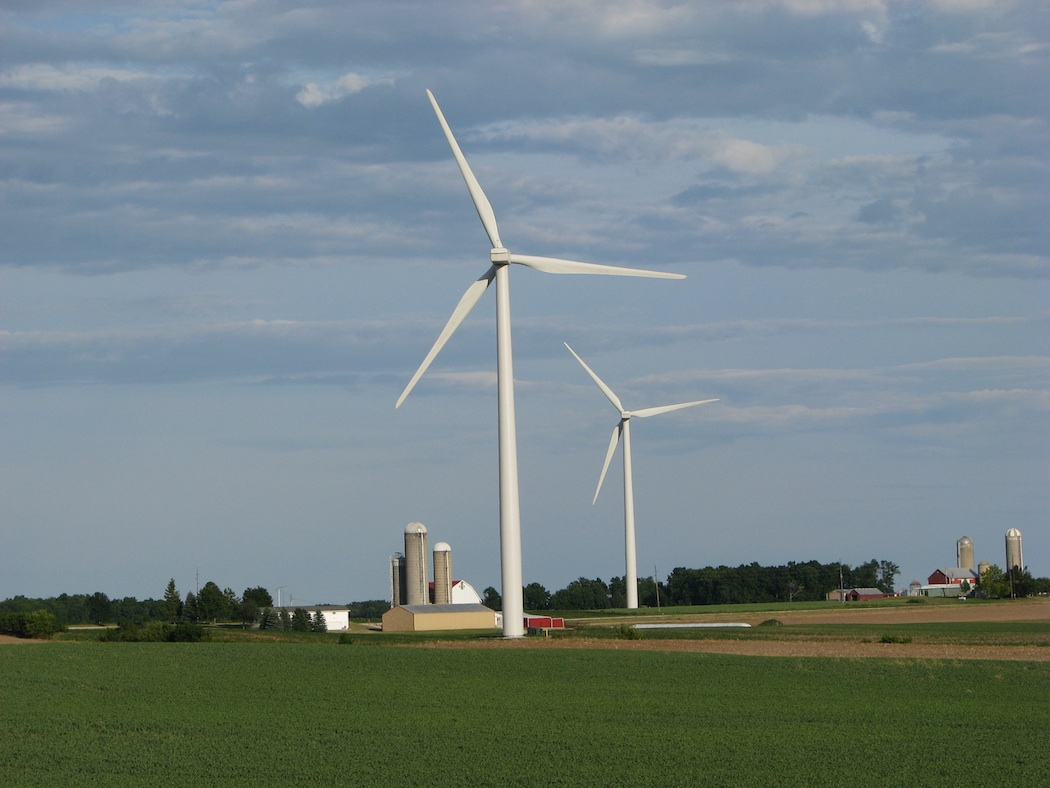
\includegraphics[height=2.5in]{files/21206}}
\hfill 
\subfigure[Aerial view of the National Wind Technology Center. 
 (Photo by Dennis Schroeder / NREL)\label{fig:20018}]
 {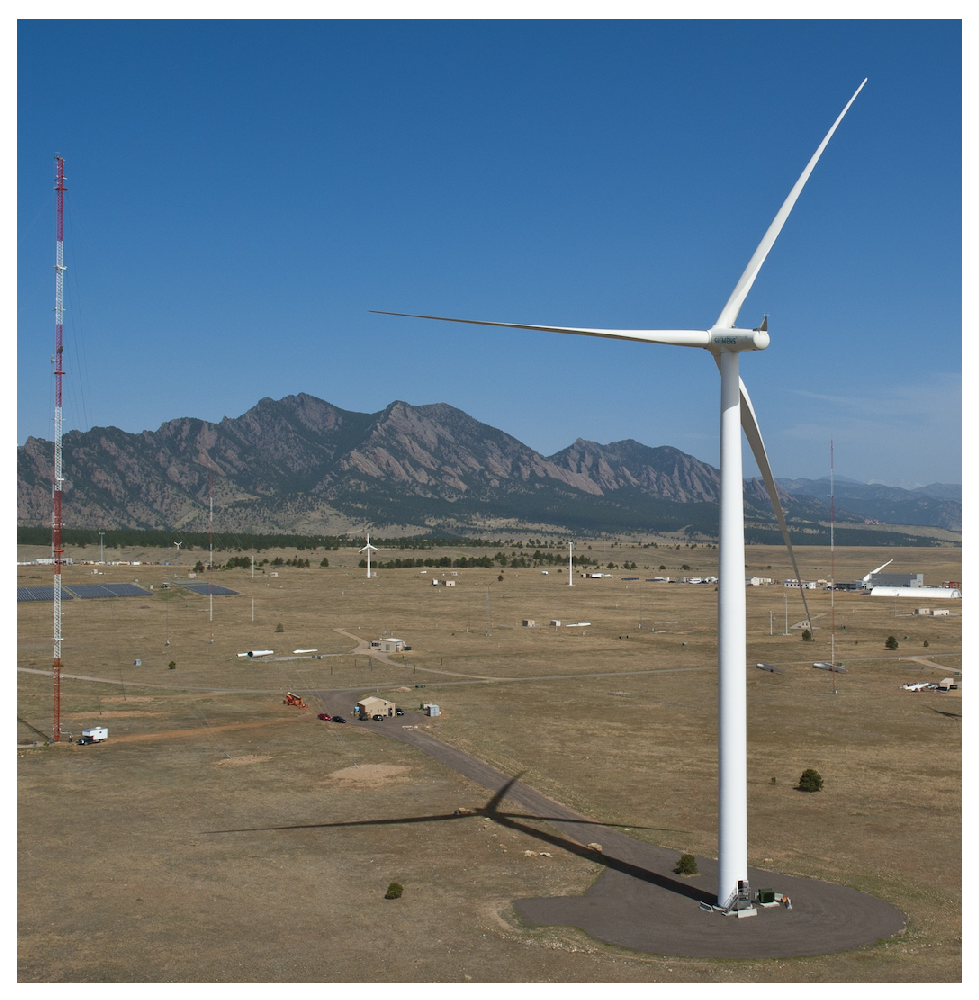
\includegraphics[height=2.5in]{files/20018}}
\hfill
\caption{NREL images}\label{fig:NRELimages}
\end{figure}
\end{verbatim}
 
\begin{figure*}[htp]
\centering
\hfill
\subfigure[Wind turbines at the Forward Wind Energy Center in Fond du Lac and Dodge Counties, Wisconsin. (Photo by Ruth Baranowski / NREL)\label{fig:21206}]{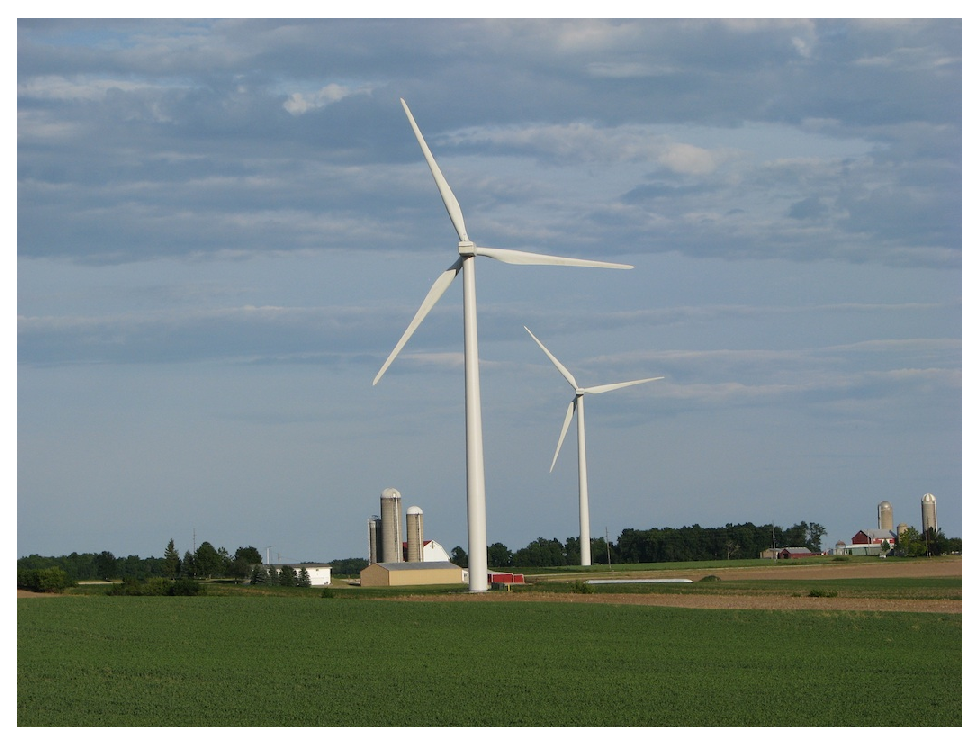
\includegraphics[height=2.5in]{files/21206.eps}}
~ %add desired spacing between images, e. g. ~, \quad, \qquad etc. (or a blank line to force the subfigure onto a new line)
\hfill
\subfigure[Aerial view of the National Wind Technology Center. (Photo by Dennis Schroeder / NREL)\label{fig:20018}]{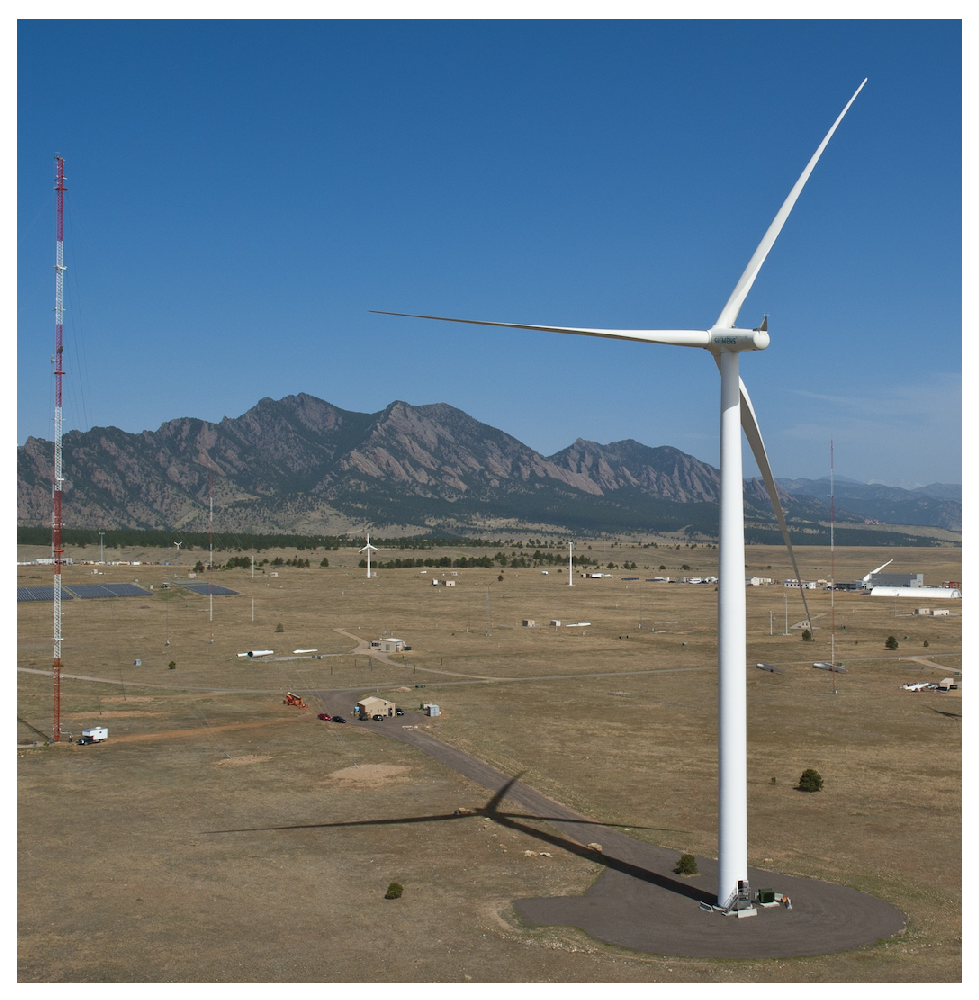
\includegraphics[height=2.5in]{files/20018.eps}}
\hfill
\caption{NREL images}\label{fig:NRELimages}
\end{figure*}

If a subfigure is split over two lines using \verb+\\+, make sure those symbols are on their own line.

\section{Lists}

To make lists with automatic numbering, use the \texttt{enumerate} environment:

\begin{enumerate}
\item Like this,
\item and like this.
\end{enumerate}
\dots or bullet points \dots
\begin{itemize}
\item Like this,
\item and like this.
\end{itemize}

\section{Computer code}
The \texttt{lstlisting} package has been loaded.

\section{Creating a file structure}
\label{sec:FileStructure}
Use the \texttt{input} command to import other files into your main file. For example, each of the chapters in this report could be in separate files, called \emph{NRELRequirements} (Chapter 1), \emph{LatexAtNREL} (Chapter 2), and so-on. 

\begin{verbatim}
...
% content
\input{NRELRequirements}
\input{LatexAtNREL}
\chapter{Some LaTeX examples}
This chapter includes examples of how to do common tasks using LaTeX{}. Although most users will be familiar with these commands and environments, these serve as a) a test of the class file and conversion process, and b) examples that are known to work with the class and conversion process. So, when all else fails, users can copy these examples and tailor them to their particular case.

\section{Headings}
LaTeX{} allows a very simple definition of the document's structure. This document has the following structure:
\begin{itemize}
\item Chapter 1: what is LaTeX?
\begin{itemize}
\item Section 1: Headings
\item Section 2: Floats
\item Section 3: Mathematics
\item Section 4: Lists
\end{itemize}
\item etc. \ldots
\end{itemize}

\subsection{Chapter}
To define a new chapter, simply write \verb+\chapter{What is LaTeX?}+.

To use chapters, pass the \texttt{memoir}, \texttt{book}, or \texttt{report} option to \emph{nrel.cls} (see Section \ref{sec:nrel.cls.options}).

\subsection{Sections}
If Chapters are the highest level headings in a document, sections come next, followed by subsections. Although there don't have to be chapters in a document, a LaTeX document does need to have Sections.

So: 

\begin{verbatim}
\section{Headings}
LaTeX{} allows a very simple definition of the document's structure. 
This document has the following structure:
...
\subsection{Chapter}

\end{verbatim}

\section{Body text}
Body text does not need to be specially identified in LaTeX{}. Non-printing comments are identified in the source document(s) using the \% symbol.

\section{Mathematics}

LaTeX is great at typesetting mathematics. The following example is taken from the \href{www.writelatex.com}{www.writelatex.com} website:

\begin{quote}
Making inline equations is easy. Let $X_1, X_2, \ldots, X_n$ be a sequence of independent and identically distributed random variables with $\textrm{E}[X_i] = \mu$ and $\textrm{Var}[X_i] = \sigma^2 < \infty$, and let
$$S_n = \frac{X_1 + X_2 + \cdots + X_n}{n}
 = \frac{1}{n}\sum_{i}^{n} X_i$$
denote their mean. Then as $n$ approaches infinity, the random variables $\sqrt{n}(S_n - \mu)$ converge in distribution to a normal $\mathcal{N}(0, \sigma^2)$.
\end{quote}

Alternatively, if numbered equations are required, use the \texttt{equation} environment. For example:

\begin{verbatim}
\begin{equation}
y = mx +c \textrm{.}
\label{eqn:line}
\end{equation}
\end{verbatim}

would give:

\begin{equation}
y = mx+c \textrm{.}
\label{eqn:line}
\end{equation}

\section{Cross references}
Use labels and references to refer back and forth to figures, equations, tables and sections. For example, \verb+Eqn. \ref{eqn:line}+ gives a reference to Eqn. \ref{eqn:line}.

\section{Floats}
Floats are images, tables or other pieces of the document that are free to move to the best place in the document for them. Literally, they `float'. The two most common floats are the tabular environment (for tables) and the figure environment for figures.

\subsection{Tables}
Use the \texttt{tabular} environment to produce basic tables. Table~\ref{tab:widgets} is produced using this code: 

\begin{verbatim}
\begin{table}[!h]
\centering
\caption{An example table.}\label{tab:widgets}
\begin{tabular}{lr}
Item & Quantity \\\hline
Widgets & 42 \\
Gadgets & 13
\end{tabular}
\end{table}
\end{verbatim}

\begin{table}[!h]
\centering
\caption{An example table.}\label{tab:widgets}
\begin{tabular}{lr}
Item & Quantity \\\hline
Widgets & 42 \\
Gadgets & 13
\end{tabular}
\end{table}

Resist the temptation to stop table rows early. If all of the delimiters  (\&) are included in each row, the table will be complete and will better translate to RTF later.

\subsection{Figures}
To include a figure in a document, use the \texttt{figure} environment and the \texttt{includegraphics} command.

\begin{verbatim}
\begin{figure}
\includegraphics[width=\textwidth]{figure's-file-name}
\caption{Caption goes here.}\label{fig:figuresLabel}
\end{figure}
\end{verbatim}

\subsection{Subfigures}
Subfigures are implemented using the \texttt{subfig} package. Although this package is deprecated (apparently \texttt{subcaption} is now the preferred package), it plays fairly nicely with \texttt{latex2rtf} so will be used for the foreseeable future. 

The \texttt{label}s in the example below allow us to make references using the \texttt{ref} command, both to the overall figure (Figure \ref{fig:NRELimages}) and the subfigures (Figures \ref{fig:21206} and \ref{fig:20018}) directly. Unfortunately, \texttt{latex2rtf} does not allow multiple \texttt{label}s in a Figure environment, and so only the first label will be kept: therefore, it's best to just use a single label in any one \texttt{figure} environment.

\begin{verbatim}
\begin{figure}
\centering
\hfill
\subfigure[Wind turbines at the Forward Wind Energy Center in Fond du Lac 
 and Dodge Counties, Wisconsin. (Photo by Ruth Baranowski / NREL)
 \label{fig:21206}]{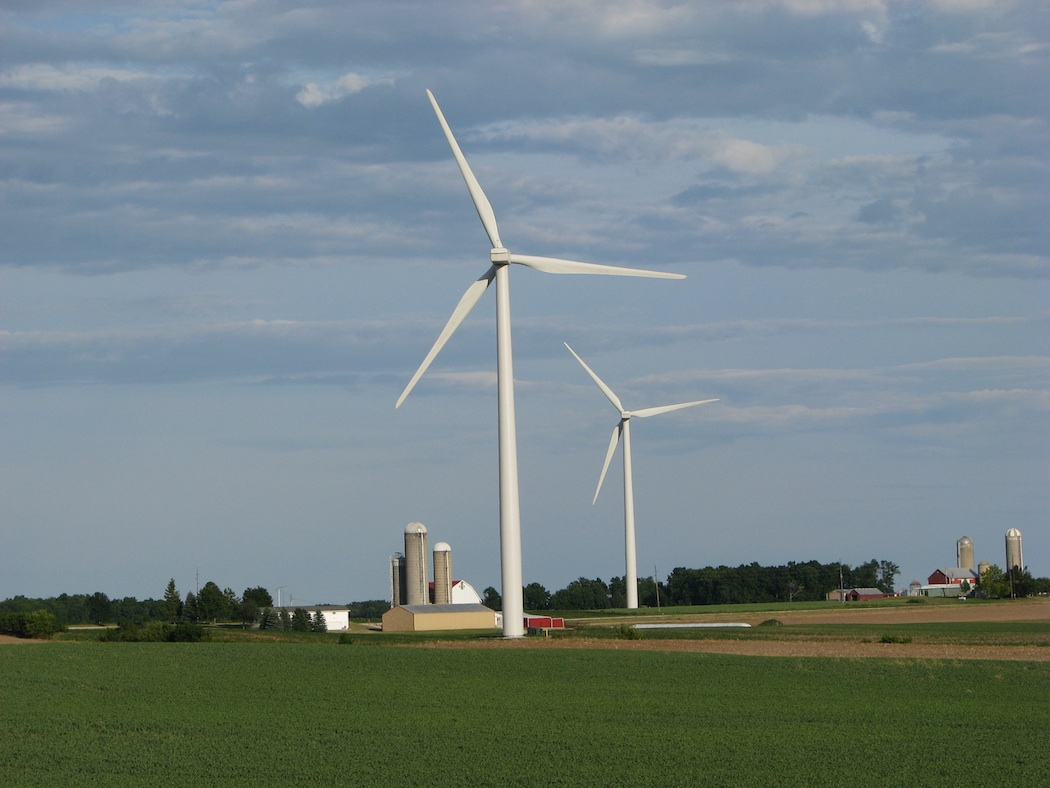
\includegraphics[height=2.5in]{files/21206}}
\hfill 
\subfigure[Aerial view of the National Wind Technology Center. 
 (Photo by Dennis Schroeder / NREL)\label{fig:20018}]
 {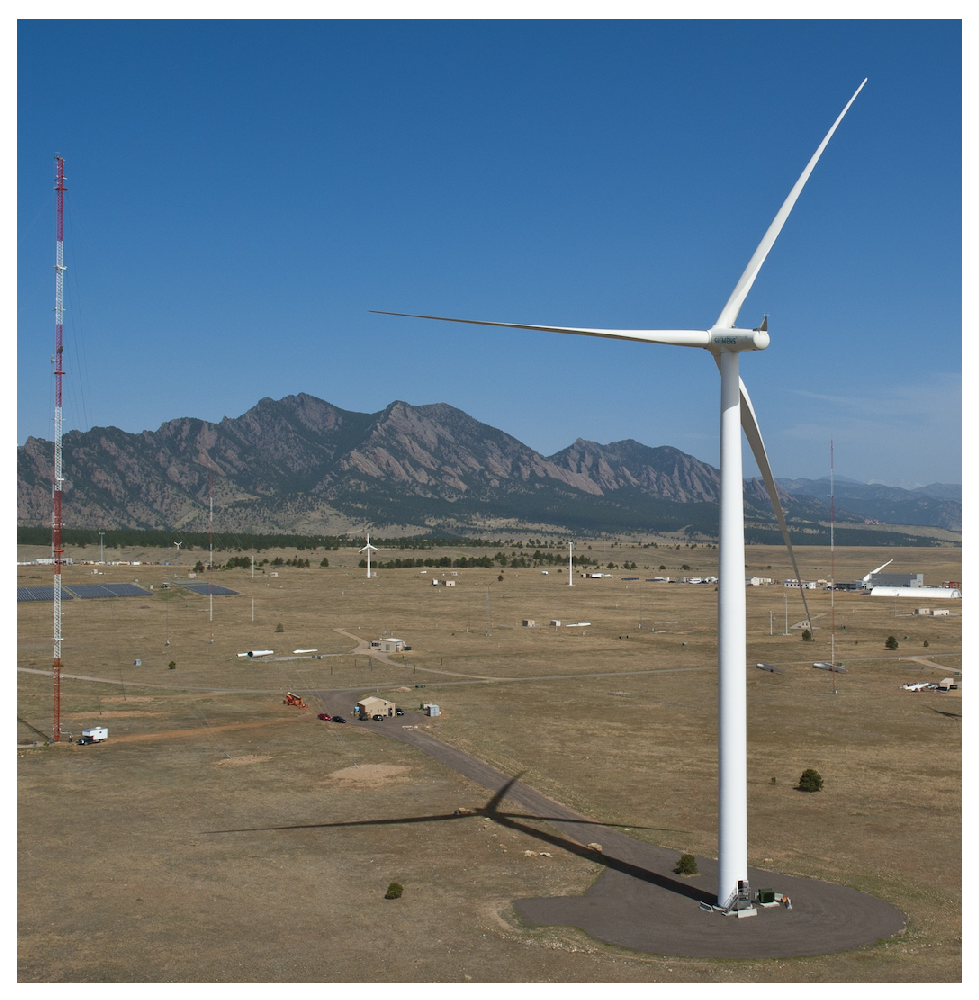
\includegraphics[height=2.5in]{files/20018}}
\hfill
\caption{NREL images}\label{fig:NRELimages}
\end{figure}
\end{verbatim}
 
\begin{figure*}[htp]
\centering
\hfill
\subfigure[Wind turbines at the Forward Wind Energy Center in Fond du Lac and Dodge Counties, Wisconsin. (Photo by Ruth Baranowski / NREL)\label{fig:21206}]{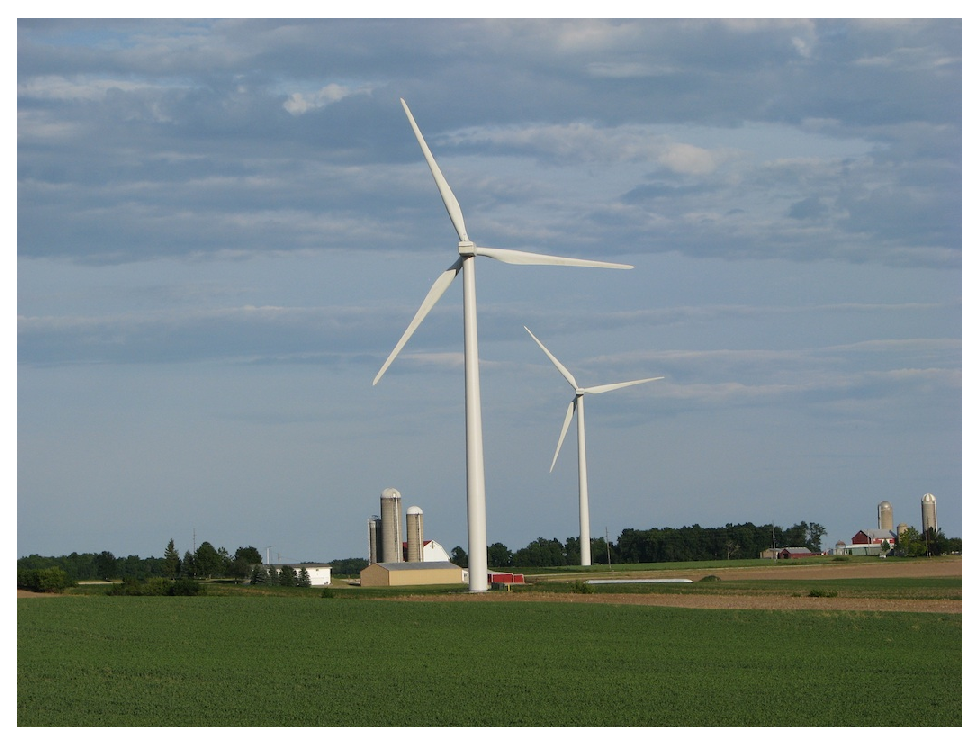
\includegraphics[height=2.5in]{files/21206.eps}}
~ %add desired spacing between images, e. g. ~, \quad, \qquad etc. (or a blank line to force the subfigure onto a new line)
\hfill
\subfigure[Aerial view of the National Wind Technology Center. (Photo by Dennis Schroeder / NREL)\label{fig:20018}]{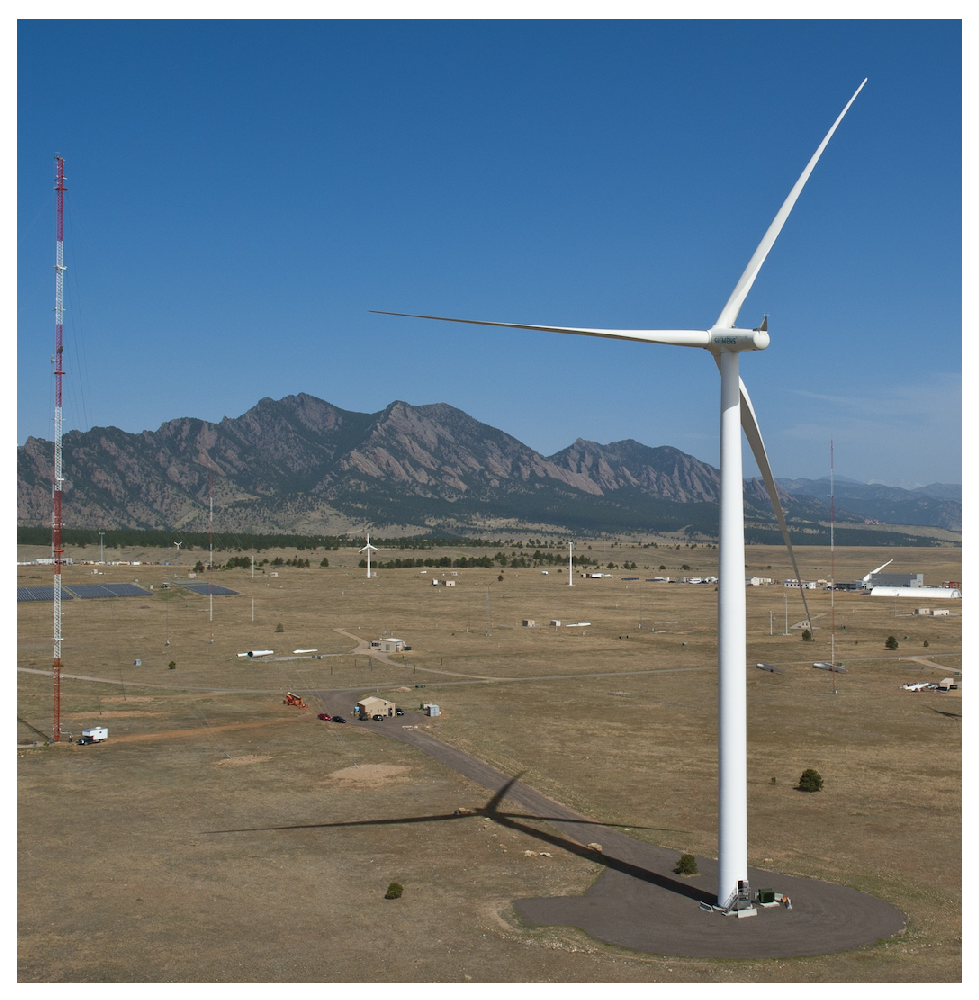
\includegraphics[height=2.5in]{files/20018.eps}}
\hfill
\caption{NREL images}\label{fig:NRELimages}
\end{figure*}

If a subfigure is split over two lines using \verb+\\+, make sure those symbols are on their own line.

\section{Lists}

To make lists with automatic numbering, use the \texttt{enumerate} environment:

\begin{enumerate}
\item Like this,
\item and like this.
\end{enumerate}
\dots or bullet points \dots
\begin{itemize}
\item Like this,
\item and like this.
\end{itemize}

\section{Computer code}
The \texttt{lstlisting} package has been loaded.

\section{Creating a file structure}
\label{sec:FileStructure}
Use the \texttt{input} command to import other files into your main file. For example, each of the chapters in this report could be in separate files, called \emph{NRELRequirements} (Chapter 1), \emph{LatexAtNREL} (Chapter 2), and so-on. 

\begin{verbatim}
...
% content
\input{NRELRequirements}
\input{LatexAtNREL}
\input{LatexExamples}
\input{ConvertingToDoc}
...
\end{verbatim}

\input{ConvertingToDoc}
...
\end{verbatim}

\input{ConvertingToDoc}
...
\end{verbatim}

\input{ConvertingToDoc}
...
\end{verbatim}
